\documentclass[11pt,letterpaper]{report}
\usepackage[utf8]{inputenc}
\usepackage[T1]{fontenc}
\usepackage[spanish]{babel}
\usepackage{amsmath}
\usepackage{amsfonts}
\usepackage{amssymb}
\usepackage{makeidx}
\usepackage{makeidx}
\usepackage{graphicx}
\usepackage{mdframed}
\usepackage{xcolor}
\usepackage[left=2.00cm, right=2.00cm]{geometry}
\author{Dr. Alejandro Rodr\'iguez}
\title{Clases Practicas}
\date{Universidad Tecnol\'ogica de Iz\'ucar de Matamoros}


\newenvironment{problem}[2][Ejercicio]
{ \begin{mdframed}[] \textbf{#1 #2} \\}
    {  \end{mdframed}}




\begin{document}
  \maketitle
  \newpage

  \chapter*{Nota preliminar}
    Los ejercicios a continuación tiene como propósito ayudarle al estudiante a reconocer debilidades y fortalezas propias en el conocimiento de la materia. Se le recomienda a los estudiantes investigar de forma autodidacta ante las dudas, de modo que desarrolle la capacidad de búsqueda y solución de los problemas planteados.

    Algunos términos y conceptos difieren entre autores y documentos disponibles en la red o en la biblioteca, por favor sea sensible y comprensible con esto. Ante cualquier duda no dude en preguntar.

    Cualquier error encontrada en este texto, por favor hágalo saber al profesor de la asignatura.
    PD: También se aceptan sugerencias.


  \chapter{Estad\'istica Descriptiva}
    \section{Introducción a la estadística}

      \subsection*{Ejercicio 1}
        Con sus propias palabras defina: Estadística, Estadística Descriptiva y Datos en la estadística.
      \subsection*{Ejercicio 2}
        ¿Que son las variables estadísticas?.
      \subsection*{Ejercicio 3}
         Dada los siguientes datos, clasifique a que tipo de variable estadística pertenece.
        \begin{itemize}
      	  \item Masculino, Femenino
          \item 3.45Kg, 45.6Kg, 105.0Kg
          \item -2, 1000, -3045, 0
          \item Soltero, Casado, Viudo, Divorciado, Unión Libre
          \item Número de Hijos
          \item Estado Civil
          \item Números enteros positivos
          \item Números enteros negativos
          \item Verde, Amarillo, Rojo
          \item ¿Está vacunado?, ¿Sí o No?
        \end{itemize}
      \subsection*{Ejercicio 4}
        Confeccione una tabla de datos que contenga cada uno de los tipos de variables que usted desee.


    \section{Población, muestra y muestreo}
      \subsection*{Ejercicio 6}
        Defina con sus palabras: Universo o Población, Muestra y Elemento.
      \subsection*{Ejercicio 7}
        De los universos siguientes, ¿cuáles están definidos rigurosamente y cuáles no?¿Por qué?
        \begin{enumerate}
      	  \item [a.] Habitantes de la ciudad de Puebla mayores de 18 años. Marzo de 1993.
      	  \item [b.] Estudiantes de Ingeniería de 2000.
      	  \item [c.] Obrero de planta permanente de la fábrica de autos Volkswagen.
      	  \item [d.] Los números primos menores que 20.
      	  \item [e.] Viviendas con más de dos recamaras en la Ciudad Izúcar de Matamoros.
        \end{enumerate}
      \subsection*{Ejercicio 8}
        Dé una posible muestra de tamaño 4 de cada una de las siguientes poblaciones.
        \begin{itemize}
            \item[a.] Todo el personal de una clínica.
            \item[b.] Todos los ríos de México.
            \item[c.] Todos los estudiantes en su colegio o universidad.
            \item[d.] Todas las calificaciones promedio de los estudiantes en su
            colegio o universidad.
        \end{itemize}

      \subsection*{Ejercicio 9}
        Se desea tomar una muestra aleatoria estratificada de las personas mayores de edad de un municipio, cuyos estratos son los siguientes intervalos de edades, en años: de 18 a 30, de 31 a 45, de 46 a 60 y mayores de 60. En el primer intervalo hay 7500 personas, en el segundo hay 8400, en el tercero 5700 y en el cuarto 3000. Calcule el tamaño de la muestra total y su composición, sabiendo que el muestreo se hace de forma proporcional y se han elegido al azar 375 personas del primer estrato.
      \subsection*{Ejercicio 10}
        En un pueblo habitan 700 hombres adultos, 800 mujeres adultas y 500 menores. De él se quiere seleccionar una muestra de 80 personas, utilizando, para ello, muestreo estratificado y se  tomaran de forma proporcional proporcional. ¿Cuál será la composición que debe tener dicha muestra?
      \subsection*{Ejercicio 11}
        Una ganadería tiene 3000 vacas. Se quiere extraer una muestra de 120. Explica cómo se obtiene
        dicha muestra:
        a) Mediante muestreo aleatorio simple.
        b) Mediante muestreo aleatorio sistemático.
    \section{Distribución de frecuencias y su representación gráfica}
      \subsection*{Ejercicio 12}
        Dada la distribución siguiente, constrúyase una tabla estadística en la que aparezcan las frecuencias absolutas, las frecuencias relativas y las frecuencias acumuladas relativas crecientes:
        \begin{table}[!h]
          \centering
          \begin{tabular}{|c|cccccc|}
              \hline
              $x_i$ & 1 & 2 & 3 & 4 & 5 & 6  \\
              \hline
              $n_i$ & 5 & 7 & 9 & 6 & 7 & 6  \\
              \hline
          \end{tabular}
        \end{table}
      \subsection*{Ejercicio 13}
        Los datos que se dan a continuación corresponden a los pesos en Kg. de ochenta personas:\\

        (a) Obténgase una distribución de datos en intervalos de amplitud 5, siendo el primer intervalo [50; 55].

        (b) Calcúlese el porcentaje de personas de peso menor que 65 Kg.

        (c) ¿Cuántas personas tienen peso mayor o igual que 70 Kg. pero menor que 85? \\

        60; 66; 77; 70; 66; 68; 57; 70; 66; 52; 75; 65; 69; 71; 58; 66; 67; 74; 61; 63; 69; 80; 59; 66; 70; 67; 78; 75; 64; 71; 81; 62; 64; 69; 68; 72; 83; 56; 65; 74; 67; 54; 65; 65; 69; 61; 67; 73; 57; 62; 67; 68; 63; 67; 71; 68; 76;
        61; 62; 63; 76; 61; 67; 67; 64; 72; 64; 73; 79; 58; 67; 71; 68; 59; 69; 70; 66; 62; 63; 66;
      \subsection*{Ejercicio 14}
        Las edades de los empleados de una determinada empresa son las que aparecen en la siguiente tabla:

        \begin{table}[!h]
          \centering
          \begin{tabular}{|c|c|}
              \hline
              Edad & N$^o$ empleados   \\
              \hline
              Menos de 25 & 22 \\
              Menos de 35 & 70 \\
              Menos de 45 & 121\\
              Menos de 55 & 157\\
              Menos de 65 & 184\\
              \hline
          \end{tabular}
        \end{table}

        Sabiendo que el empleado más joven tiene 18 años, escríbase la distribución de frecuencias acumuladas decrecientes (o «más de»).
      \subsection*{Ejercicio 15}
        Las temperaturas medias registradas durante el mes de mayo en Madrid, en grados centígrados, están dadas por la siguiente tabla:
        \begin{table}[!h]
            \centering
            \begin{tabular}{|c|c|c|c|c|c|c|c|c|c|c|}
                \hline
                Temperatura & 13 &14& 15& 16& 17 &18& 19& 20& 21& 22  \\
                \hline
               N.$^o$ de días &1 &1 &2 &3 &6 &8 &4 &3 &2& 1   \\
                \hline
            \end{tabular}
       \end{table}

       Constrúyase la representación gráfica correspondiente.
      \subsection*{Ejercicio 16}
         Dada la distribución de frecuencias:
         \begin{table}[!h]
             \centering
             \begin{tabular}{|c|c|}
                 \hline
                 $x_i$ & $n_i$ \\
                 \hline
                 1  & 9   \\
                 \hline
                 2  & 22  \\
                 \hline
                 3  & 13  \\
                 \hline
                 4  & 23  \\
                 \hline
                 5  & 8   \\
                 \hline
                 6  & 25  \\
                 \hline
             \end{tabular}
         \end{table}
         \\
         (a) Constrúyase una tabla en la que aparezcan frecuencias absolutas, frecuencias relativas, frecuencias acumuladas absolutas crecientes (o «menos de») y decrecientes (o «más de»).\\
         (b) Represéntese mediante un diagrama de barras la distribución dada y su correspondiente polígono de frecuencias.\\
         (c) Obténgase el polígono de frecuencias absolutas acumuladas crecientes y decrecientes.\\
      \subsection*{Ejercicio 17}
        Represéntese gráficamente la siguiente distribución de frecuencias:
        \begin{table}[!h]
            \centering
            \begin{tabular}{|c|c|}
                \hline
                $L_{i-1}-L_i$  & $n_i$\\
                \hline
                0-10& 22\\
                \hline
                10-20& 26\\
                \hline
                20-30& 92\\
                \hline
                30-40& 86\\
                \hline
                40-50& 74\\
                \hline
                50-60& 27\\
                \hline
                60-70& 12\\
                \hline
            \end{tabular}
        \end{table}
      \subsection*{Ejercicio 18}
        Encuestados cincuenta matrimonios respecto a su número de hijos, se obtuvieron los siguientes datos:\\

        2; 4; 2; 3; 1; 2; 4; 2; 3; 0; 2; 2; 2; 3; 2; 6; 2; 3; 2; 2; 3; 2; 3; 3; 4; 1; 3; 3; 4; 5; 2; 0; 3; 2; 1; 2; 3; 2; 2; 3; 1; 4; 2; 3; 2; 4; 3; 3; 2\\

        Constrúyase una tabla estadística que represente dichos datos
      \subsection*{Ejercicio 19}



    \section{Medidas de tendencia central, localización y dispersión}
      \subsection*{Ejercicio 19}
        Calculo de la media aritmética, la mediana y la moda. Se analizó el IVA que se aplica, en diversos países europeos, a la compra de obras de arte. Los resultados obtenidos fueron los siguientes:
        \begin{table}[!h]
            \begin{tabular}{|c|c|}
                \hline
                PAIS& \\
                \hline
                España &0,16\\
                Italia &0,20\\
                Bélgica& 0,06\\
                Holanda& 0,06\\
                Alemania& 0,07\\
                Portugal& 0,17\\
                Luxemburgo& 0,06\\
                Finlandia& 0,22\\
                \hline
            \end{tabular}
        \end{table}

  \chapter{Probabilidad}
    \section{Conjuntos}
      \subsection{}
        Considere el experimento de lanzar un dado. Si nos interesara el número que aparece en la cara superior, ¿Cual es el espacio muestral?. ¿.Y, si sólo estuviéramos interesados en si el número es par o impar?
      \subsection{}
        En el experimento en el cual se observa el número de bombas en uso en una sola gasolinera de seis bombas, sea A = {0, 1, 2, 3, 4}, B = {3, 4, 5, 6} y C = {1, 3, 5}
        Enuncie:
        \begin{itemize}
            \item A'
            \item A $\cup$ B
            \item A $\cap$ B
            \item A $\cup$ C
            \item A $\cap$ C
        \end{itemize}
      \subsection{}
        Cuatro universidades, 1, 2, 3 y 4, están participando en un torneo de básquetbol. En la primera ronda, 1 jugará con 2 y 3 jugará con 4. Acto seguido los ganadores jugarán por el campeonato y los dos perdedores también jugarán. Un posible resultado puede ser denotado por 1324 (1 derrota a 2 y 3 derrota a 4 en los juegos de la primera ronda y luego 1 derrota a 3 y 2 derrota a 4).
        \begin{itemize}
          \item [a)] Enumere todos los resultados en E.
          \item [b)] Que A denote el evento en que 1 gana el torneo. Enumere los resultados en A.
          \item [c)] Que B denote el evento en que 2 gana el juego de campeonato. Enumere los resultados en B.
        \end{itemize}
      \subsection{}
        Un experimento consiste en lanzar una moneda tres veces. ¿Haga el diagrama de árbol?. Determine el espacio muestral.
      \subsection{}
        Un experimento consiste en lanzar una moneda y después lanzarla una segunda vez si sale cara. Si en el primer lanzamiento sale cruz, entonces se lanza un dado una vez. ¿Haga el diagrama de árbol?. Determine el espacio muestral.
      \subsection{}
        ¿Cuántos puntos muestrales hay en el espacio muestral cuando se lanza un par de dados una vez?
      \subsection{}
        Un vendedor de viviendas ofrece a los posibles compradores de una casa a elegir entre diferentes fachadas:  Tudor, rústica, colonial y tradicional, mientras que el plano de construcción puede ser:  una planta, dos pisos y desniveles. ¿En cuántas formas diferentes puede un comprador ordenar una de estas casas?
      \subsection{}
        Si un miembro de un club que tiene 22 integrantes necesitara elegir un presidente y un tesorero, ¿de cuántas maneras diferentes se podría elegir a ambos?
    \section{Permutación y combinaciones}
      \subsection{}
        En un año se otorgará uno de tres premios (a la investigación, la enseñanza y el servicio) a algunos de los estudiantes, de un grupo de 25, de posgrado del departamento de estadística. Si cada estudiante puede recibir un premio como máximo, ¿cuántas selecciones posibles habría?
      \subsection{}
        En un club estudiantil compuesto por 50 personas se va a elegir a un presidente y a un tesorero. ¿Cuántas opciones diferentes de funcionarios son posibles si:
        \begin{itemize}
            \item [a)] no hay restricciones;
            \item [b)] A participará sólo si él es el presidente;
            \item [c)] B y C participarán juntos o no lo harán;
        \end{itemize}
      \subsection{}
        Un niño le pide a su madre que le lleve cinco cartuchos de Game-Boy TM de su colección de 10 juegos recreativos y 5 de deportes. ¿De cuántas maneras podría su madre llevarle 3 juegos recreativos y 2 de deportes?
      \subsection{}
        ¿Cuántos arreglos diferentes de letras se pueden hacer con las letras de la palabra STATISTICS?
    \section{Probabilidad condicional y Probabilidad de eventos independientes}
      \subsection{Ejemplo resuelto, calculo de probabilidades basándonos en el árbol de probabilidades.}

      En una casa hay tres llaveros A, B y C; el primero con cinco llaves, el segundo con siete y el tercero con ocho, de las que sólo una de cada llavero abre la puerta de la cochera. Se escoge al azar un llavero y, de él una llave para abrir la cochera. Se pide:
      \begin{enumerate}
          \item ¿Cuál será la probabilidad de que se acierte con la llave?
          \item ¿Cuál será la probabilidad de que el llavero escogido sea el tercero y la llave no abra?
          \item Y si la llave escogida es la correcta, ¿cuál será la probabilidad de que pertenezca al primer llavero A?
      \end{enumerate}
      \textbf{Solución:}
      Primero debemos hacer el diagrama de árbol de probabilidades, y le colocamos las probabilidades asociadas a cada evento.

      \begin{figure}[!h]
          \centering
          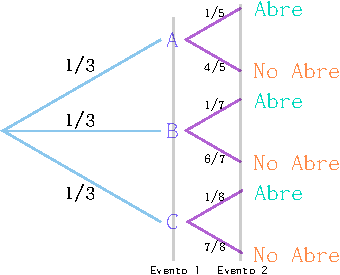
\includegraphics[width=0.5\linewidth]{images/cp2}
          \caption{Diagrama de Árbol de Probabilidades.}
          \label{fig:cp2}
      \end{figure}

      Como vemos en la Figura \ref{fig:cp2}, la probabilidad se escoger una llavero puesto que son solo tres llaveros y cada uno tiene igual probabilidad de ser escogido, la probabilidad es de $1/3$. Luego de escoger un hipotético llavero, debemos tenemos dos opciones al seleccionar cualquier llave (abre o no abre). Por tanto y tomando el llavero a a modo de ejemplo, sabemos que solo una llave de las 5 posibles pueden abrir el llavero as\'i pues la probabilidad de extraer esa llave es de $1/5$ y de no hacerlo la diferencia ($1-1/5=4/5$) que es $4/5$. De esta forma se hacen con todos los llaveros.

      Luego, cabe señalar que la probabilidad a lo largo de las ramas, se \textbf{multiplican} y la probabilidad de diferentes ramas del un mismo evento se \textbf{suman}, como se muestra en la Figura\ref{fig:cp1}.

      \begin{figure}[!h]
          \centering
          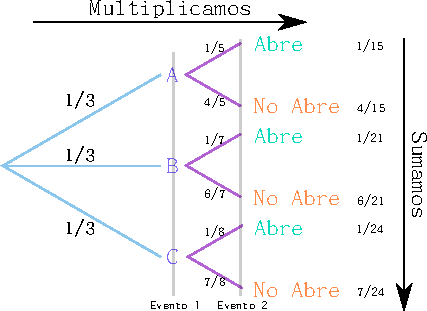
\includegraphics[width=0.5\linewidth]{images/cp1}
          \caption{La suma de las probabilidad de cada rama siempre debe sumar 1. Puesto que la probabilidad total es 1.}
          \label{fig:cp1}
      \end{figure}


      De esta forma estamos en condiciones de resolver cada una de las interrogantes, recordemos la pregunta. Se escoge al azar un llavero y, de él una llave para abrir la cochera. Se pide:

      1. ¿Cuál será la probabilidad de que se acierte con la llave?

      Calculamos la probabilidad de escoger la llave que abre en cada caso y luego las sumamos.

      $$P(Abrir)=\dfrac{1}{3}\times\dfrac{1}{5}+\dfrac{1}{3}\times\dfrac{1}{7}+\dfrac{1}{3}\times\dfrac{1}{8}=0.1559$$
      Lo cual equivale a 15.59\%.

      2. ¿Cuál será la probabilidad de que el llavero escogido sea el tercero y la llave no abra?

      Calculamos la probabilidad de escoger la una llave que \textbf{NO} abra del llavero \textbf{C}, es decir multiplicamos $1/3$ que corresponde a la probabilidad de escoger el llavero \textbf{C} y lo multiplicamos por $7/8$ que representan la probabilidad de que la llave escogida de este llavero no abra.

      $$P(NoAbrirC)=\dfrac{1}{3}\times\dfrac{7}{8}=0.2917$$
      Lo cual equivale a 29.17\%.

      3. Y si la llave escogida es la correcta, ¿cuál será la probabilidad de que pertenezca al primer llavero A?

      Acá la probabilidad esta condicionada. Ya sabemos de antemano (a priori) que la llave es la correcta, y esto condiciona la probabilidad de que sea del llavero \textbf{A}. Planteemos la ecuación:
      $$P(AbreCondicionado)=\dfrac{P(llaveroA)}{P(TotalAbre)}=\dfrac{\dfrac{1}{3}\times\dfrac{1}{5}}{\dfrac{1}{3}\times\dfrac{1}{5}+\dfrac{1}{3}\times\dfrac{1}{7}+\dfrac{1}{3}\times\dfrac{1}{8}}=0.4275$$

      \subsection{Ejemplo resuelto, calculo de probabilidades basándonos en el Diagrama de Venn}
        En una ciudad, el 40\% de la población tiene cabellos castaños, el 25\% tiene ojos castaños y el 15\% tiene cabellos y ojos castaños. Se escoge una persona al azar:
        \begin{itemize}
            \item Si tiene los cabellos castaños, ¿cuál es la probabilidad de que tenga también ojos castaños?
            \item Si tiene ojos castaños, ¿cuál es la probabilidad de que no tenga cabellos castaños?
            \item ¿Cuál es la probabilidad de que no tenga cabellos ni ojos castaños?
        \end{itemize}

        \textbf{Solución}

        Para resolver este ejercicio nos vamos a apoyar en el diagrama de Venn y de una Tabla. Ambos recursos pueden ser usados de forma indistinta (puede usar uno o el otro, con uno solo se puede resolver el problema). Nosotros haremos el ejercicio con ambos recursos para ilustrar su uso he importancia.

        Primero debemos hace el diagrama de Venn y la tabla de probabilidades para esbozar el problema. El diagrama de ven debe quedar como en la Figura\ref{fig:cp3}. Véase que \textbf{E} representa el espacio muestral que es el 100\% o el total o probabilidad $1$ (todo esto es lo mismo). Luego representamos ambas proposiciones. Una esfera (Roja) representa la posicionan con cabello castaño, la cual denotaremos como (CC), y la otra esfera de color azul, la población de ojos castaños, que denotaremos como (OC).


        \begin{figure}[!h]
            \centering
            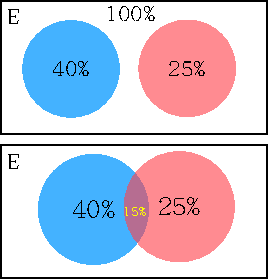
\includegraphics[width=0.4\linewidth]{images/cp3}
            \caption{Proporciones de cabello y ojos castaños por separado y luego como se unen y esta proporci\'on es del 15\%. Quiere decir que parte de las personas que tienen cabello castaño tienen también los ojos castaños y viceversa.}
            \label{fig:cp3}
        \end{figure}


        Como se puede observar la intercepción correspondes a las poblaciones de persona que tienen, tanto el cabello como los ojos castaños, la cual representa el 15\%. En la Tabla\ref*{tab:prob} lo representamos de la siguiente forma. Se hace notar que tanto CC' como OC' representan las personas con cabello castaño que no tienen ojos castaños, es decir tiene el cabello castaño pero los ojos de otro color y lo mismo ocurre con el grupo de personas que solamente tienen los ojos castaños.

        \begin{table}[!h]
            \centering
            \caption{Tabla de Probabilidades}

            \begin{tabular}{c|cc|c}
                 & PeloC & PeloC' & Total \\
                \hline
                OjoC & 15 &  & 25 \\
                OjoC' &  &  &  \\
                \hline
                Total & 40 &  & 100 \\
            \end{tabular}

            \label{tab:prob}
        \end{table}

        Para completar la tabla y re-dibujar el diagrama de Venn debemos analizar los datos. Si del 40\% que representan personas con CC el 15\% de personas representan a los que tienen tanto el CC como los OC entonces $40-15=25$ que representan las personas que tienen el cabello castano y los ojos de otro color. Siguiendo esta lógica, calculamos las personas que tienen los OC y el cabello de otro color $25-15= 10$. Llegado a este punto podemos decir que, si le restamos al 100\% de la población el 40\% que equivale a las personas con CC, obtendremos un 40\% equivalente a las personas con el cabello de otro color sin importar el color de los ojos de igual forma si restamos al 100\% de la población el 25\% equivalente a personas con OC obtendremos un 75\% equivalente a personas con ojos de otro color sin importar el color del cabello. Quedando la tabla de la siguiente forma:

        \begin{table}[!h]
          \centering
          \caption{Tabla de Probabilidades}

            \begin{tabular}{c|cc|c}
              & PeloC & PeloC' & Total \\
              \hline
              OjoC & 15 & 10 & 25 \\
              OjoC' & 25 & 50 & 75  \\
              \hline
              Total & 40 & 60 & 100 \\
            \end{tabular}
          \label{tab:probb}
        \end{table}

      De igual forma se pude apreciar en el diagrama de Venn como de fácil se pueden hacer todas estas inferencias que luego ayudan a resolver los ejercicios.

      \begin{figure}
          \centering
          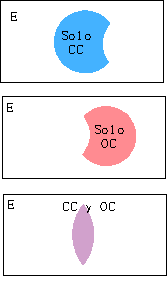
\includegraphics[width=0.4\linewidth]{images/cp4}
          \caption{Como lucen las distintas proporciones, las relaciones reales se pueden consultar en la tabla. }
          \label{fig:cp4}
      \end{figure}


      Ahora si vamos a resolver las preguntas.

      Se escoge una persona al azar:
      \begin{itemize}
          \item[a)] Si tiene los cabellos castaños, ¿cuál es la probabilidad de que tenga también ojos castaños?
          \item[b)] Si tiene ojos castaños, ¿cuál es la probabilidad de que no tenga cabellos castaños?
          \item[c)] ¿Cuál es la probabilidad de que no tenga cabellos ni ojos castaños?
      \end{itemize}


         a) Si tiene los cabellos castaños, ¿cuál es la probabilidad de que tenga también ojos castaños?

         $$P(OC)=\dfrac{15}{40}=0.375$$
         que equivale al 37.5\%


         b) Si tiene ojos castaños, ¿cuál es la probabilidad de que no tenga cabellos  castaños?
         $$P(PeloNoCastano/OjosCastano)=\dfrac{10}{25}=0.4$$

         c) ¿Cuál es la probabilidad de que no tenga cabellos ni ojos castaños?

         $$P(NiPeloNiOjosCastanos)=\dfrac{50}{100}=0.5$$
         Se divide entre 100 porque es el 100\%.

         \textbf{NOTA FINAL:} Vea como empleamos por ciento (\%) todo el tiempo. Esto es porque el por ciento y la probabilidad guardan relación donde el $100\% = Probabilida \quad 1$


      \subsection{}%64
        La probabilidad de que un vuelo programado normalmente salga a tiempo es P(D) = 0.83, la probabilidad de que llegue a tiempo es P(A) = 0.82 y la probabilidad de que salga y llegue a tiempo es P(D $\cap$ A) = 0.78. Calcule la probabilidad de que un avión.
        a) llegue a tiempo, dado que salió a tiempo;
        b) salió a tiempo, dado que llegó a tiempo.

      \subsection{}%64
        Considere un proceso industrial en el ramo textil, en el que se producen listones de una tela específica. Los listones pueden resultar con defectos en dos de sus características: la longitud y la textura. En el segundo caso el proceso de identificación es muy complicado. A partir de información histórica del proceso se sabe que 10\% de los listones no pasan la prueba de longitud, que 5\% no pasan la prueba de textura y que sólo 0.8\% no pasan ninguna de las dos pruebas. Si en el proceso se elige un listón al azar y una medición rápida identifica que no pasa la prueba de longitud, ¿cuál es la probabilidad de que la textura esté defectuosa?
      \subsection{}%Ejercicios%20y%20problemas%20de%20probabilidad%20condicionada.pdf
        En una ciudad, el 40\% de la población tiene cabellos castaños, el 25\% tiene ojos castaños y el 15\% tiene cabellos y ojos castaños. Se escoge una persona al azar:
        \begin{enumerate}
            \item Si tiene los cabellos castaños, ¿cuál es la probabilidad de que tenga también ojos castaños?
            \item Si tiene ojos castaños, ¿cuál es la probabilidad de que no tenga cabellos castaños?
            \item ¿Cuál es la probabilidad de que no tenga cabellos ni ojos castaños?
        \end{enumerate}

    \section{Prueba F Fisheren}
      \subsection{}
        Encuentra los valores de $F_{0.01}$ para cada uno de los siguientes grados de libertad.
        \begin{enumerate}
            \item $\nu_1=5$ y $\nu_2=5$
            \item $\nu_1=5$ y $\nu_2=12$
            \item $\nu_1=12$ y $\nu_2=20$
        \end{enumerate}

        %df1=5  and  df2=5   S11.0
        %df1=5  and  df2=12  S 5.06
        %df1=12  and  df2=20 S 3.23
      \subsection{}
        Encuentra los valores de $F_{0.05}$ para cada uno de los siguientes grados de libertad.
        \begin{enumerate}
            \item $\nu_1=6$ y $\nu_2=6$
            \item $\nu_1=6$ y $\nu_2=12$
            \item $\nu_1=12$ y $\nu_2=30$
        \end{enumerate}
        %Find  F0.05  for each of the following degrees of freedom.
        %df1=6  and  df2=6    S
        %df1=6  and  df2=12   S
        %df1=12  and  df2=30  S
      \subsection{}
        Encuentra los valores de $F_{0.95}$ para cada uno de los siguientes grados de libertad.
        \begin{enumerate}
            \item $\nu_1=6$ y $\nu_2=6$
            \item $\nu_1=6$ y $\nu_2=12$
            \item $\nu_1=12$ y $\nu_2=30$
        \end{enumerate}
        %Find  F0.95  for each of the following degrees of freedom.
        %df1=6  and  df2=6    S
        %df1=6  and  df2=12   S
        %df1=12  and  df2=30  S
      \subsection{}%4
         Encuentra los valores de $F_{0.90}$ para cada uno de los siguientes grados de libertad.
        \begin{enumerate}
            \item $\nu_1=5$ y $\nu_2=5$
            \item $\nu_1=5$ y $\nu_2=12$
            \item $\nu_1=12$ y $\nu_2=20$
        \end{enumerate}

        %df1=5  and  df2=5
        %df1=5  and  df2=12
        %df1=12  and  df2=20
      %\subsection{}%5
      %  Para $\nu_1=7$, $\nu_2=10$ y $\alpha=0.05$ y encuentra:
      %  \begin{enumerate}
      %      \item $F_\alpha$
      %      \item $F_{1-\alpha}$
      %      \item $F_{\alpha/2}$
      %      \item $F_{1-\alpha/2}$
      %  \end{enumerate}

        %For  df1=7 ,  df2=10  and  α=0.05 , find
        %Fα
        %F1−α
        %Fα/2
        %F1−α/2
      %\subsection{}%6
      %  Para $\nu_1=15$, $\nu_2=8$ y $\alpha=0.01$ y encuentra:
      %  \begin{enumerate}
      %      \item $F_\alpha$
      %      \item $F_{1-\alpha}$
      %      \item $F_{\alpha/2}$
      %      \item $F_{1-\alpha/2}$
      %  \end{enumerate}
        %For  df1=15 ,  df2=8  and  α=0.01 , find
        %Fα
        %F1−α
        %Fα/2
        %F1−α/2
      \subsection{}%7
        Para las siguientes dos muestras:
        \begin{table}[!h]
          \begin{tabular}{cc}
              Muestra 1:&$\{$ 8, 2, 11, 0, -2 $\}$\\
              Muestra 2:&$\{$-2, 0, 0, 0, 2, 4, -1$\}$
          \end{tabular}
        \end{table}

         encuentre:

         \begin{enumerate}
           \item Tamaño de la muestra
           \item Media
           \item Varianza
         \end{enumerate}
         %For each of the two samples
         %Sample 1:{8,2,11,0,−2}Sample 2:{−2,0,0,0,2,4,−1}(11.E.1)
         %find
       \subsection{}%8
         Para las siguientes dos muestras:
         \begin{table}[!h]
             \begin{tabular}{cc}
                 Muestra 1:&$\{$0.8, 1.2, 1.1, 0.8, -2.0 $\}$\\
                 Muestra 2:&$\{$-2.0, 0.0, 0.7, 0.8, 2.2, 4.1, -1.9$\}$
             \end{tabular}
         \end{table}

         encuentre:

         \begin{enumerate}
             \item Tamaño de la muestra
             \item Media
             \item Varianza
         \end{enumerate}
         %For each of the two samples
         %Sample 1:{0.8,1.2,1.1,0.8,−2.0}Sample 2:{−2.0,0.0,0.7,0.8,2.2,4.1,−1.9}(11.E.2)
         %find
         %the sample size
         %the sample mean
         %the sample variance
       \subsection{}%9
         Dos muestra tomadas de dos poblaciones de distribución normal nos arroja la siguiente información:


         \begin{table}[!h]
             \begin{tabular}{ccc}
                 Sample &	Sample Size	&Sample Variance\\
                 \hline
                 1	 & $n_1 = 16$ & 	 $s^2_1 = 53$ \\
                 2	 & $n_2 = 21$ & 	 $s^2_2 = 32$  \\
             \end{tabular}
         \end{table}

         Encuentre:

         \begin{enumerate}
             \item Encuentre   $F=s^2_1/s^2_2$
             \item Encuentre los grados de libertad $\nu_1$  y  $\nu_2$.
             \item Encuentre  $F_{0.05}$  empleando $\nu_1$  y  $\nu_2$ calculado anteriormente.
             \item Con una significancia del 5\%, evalúe la hipótesis: $H_0:\sigma^2_1 = \sigma^2_2$ vs $H_a: \sigma^2_1 >\sigma^2_2$.
         \end{enumerate}
         % Two random samples taken from two normal populations yielded the following information:
         %Sample	Sample Size	Sample Variance
         %1	 n1=16 	 s21=53
         %2	 n2=21 	 s22=32
         %Find the statistic  F=s21/s22
         %Find the degrees of freedom  df1  and  df2 .
         %Find  F0.05  using  df1  and  df2  computed above.
         %Perform the test the hypotheses  H0:α21=α22vsHa:α21>α22  at the  5%  level of significance.


       \subsection{}%10
         Dos muestra tomadas de dos poblaciones de distribución normal nos arroja la siguiente información:

         \begin{table}[!h]
             \begin{tabular}{ccc}
                 Sample &	Sample Size	&Sample Variance\\
                 \hline
                 1	 & $n_1 = 11$ & 	 $s^2_1 = 61$ \\
                 2	 & $n_2 = 8$ & 	 $s^2_2 = 44$  \\
             \end{tabular}
         \end{table}

         Encuentre:

         \begin{enumerate}
             \item Encuentre   $F=s^2_1/s^2_2$
             \item Encuentre los grados de libertad $\nu_1$  y  $\nu_2$.
             \item Encuentre  $F_{0.05}$  empleando $\nu_1$  y  $\nu_2$ calculado anteriormente.
             \item Con una significancia del 5\%, evalúe la hipótesis: $H_0:\sigma^2_1 = \sigma^2_2$ vs $H_a: \sigma^2_1 >\sigma^2_2$.
         \end{enumerate}
         %Two random samples taken from two normal populations yielded the following information:
         %Sample	Sample Size	Sample Variance
         %1	 n1=11 	 s21=61
         %2	 n2=8 	 s22=44
         %Find the statistic  F=s21/s22 .
         %Find the degrees of freedom  df1  and  df2 .
         %Find  F0.05  using  df1  and  df2 computed above.
         %Perform the test the hypotheses  H0:α21=α22vsHa:α21>α22  at the  5%  level of significance.


       %\subsection{}%11
       %  Dos muestra tomadas de dos poblaciones de distribución normal nos arroja la siguiente información:

       %  \begin{table}[!h]
       %      \begin{tabular}{ccc}
       %          Sample &	Sample Size	&Sample Variance\\
       %          \hline
       %          1	 & $n_1 = 10$ & 	 $s^2_1 = 12$ \\
       %          2	 & $n_2 = 13$ & 	 $s^2_2 = 23$  \\
       %      \end{tabular}
       %  \end{table}
       %
       %  Encuentre:
       %
       %  \begin{enumerate}
       %      \item Encuentre   $F=s^2_1/s^2_2$
       %      \item Encuentre los grados de libertad $\nu_1$  y  $\nu_2$.
       %      \item Encuentre para $\alpha=0.5$  $F_{1-\alpha}$  empleando $\nu_1$  y  $\nu_2$ calculado anteriormente.
       %      \item Con una significancia del 5\%, evalúe la hipótesis: $H_0:\sigma^2_1 = \sigma^2_2$ vs $H_a: \sigma^2_1 <\sigma^2_2$.
       %  \end{enumerate}
         %Two random samples taken from two normal populations yielded the following information:
         %Find the statistic  F=s21/s22 .
         %Find the degrees of freedom  df1  and  df2 .
         %For  α=0.05  find  F1−α  using  df1  and  df2  computed above.
         %Perform the test the hypotheses  H0:α21=α22vsHa:α21<α22  at the  5%  level of significance.

       \subsection{}%15
         En un criadero de peces en particular, las crías de esturión japonés recién nacidas se mantienen en tanques durante varias semanas antes de transferirlas a estanques más grandes. El oxígeno disuelto en el agua del tanque se controla muy de cerca mediante un sistema electrónico y se mantiene rigurosamente en un nivel objetivo de 6,5 miligramos por litro (mg/l). El criadero de peces busca actualizar sus sistemas de monitoreo de agua para un control más estricto del oxígeno disuelto. Se evalúa un sistema nuevo contra el anterior, que se está utilizando actualmente. Se recogieron 31 muestras de agua de un tanque operado con el sistema nuevo y 16 muestras de agua de un tanque operado con el sistema antiguo, todo durante el transcurso de un día. Las muestras arrojan la siguiente información:

         \begin{table}[!ht]
             \begin{tabular}{cc}
                 Nuevo 1: n1=31 &$s^2_1$=0.0121\\
                 Viejo 2: n1=16 &$s^2_2$=0.0319
             \end{tabular}
         \end{table}

         Pruebe, con un nivel de significación del 10\%, si los datos proporcionan evidencia suficiente para concluir que el nuevo sistema proporcionará un control más estricto del oxígeno disuelto en los tanques.
       \subsection{}%16
         El riesgo de invertir en una acción se mide por la volatilidad, o la varianza, en los cambios en el precio de esa acción. Diferentes fondos mutuos tienen diferentes enfoques y ofrecen diferentes niveles de riesgo. Juan está decidiendo entre dos fondos mutuos, A y B, con rendimientos esperados similares. Para tomar una decisión final, examinó los rendimientos anuales de los dos fondos durante los últimos diez años y obtuvo la siguiente información:
         \begin{table}[!ht]
             \begin{tabular}{cc}
                 Fondo A 1: n1=10 &$s^2_1$=0.012\\
                 Fondo B 2: n1=10 &$s^2_2$=0.005
             \end{tabular}
         \end{table}

         Pruebe, al nivel de significancia del 5\%, si los datos proporcionan evidencia suficiente para concluir que los dos fondos mutuos ofrecen diferentes niveles de riesgo.
       \subsection{}%17
         Un fabricante de computadoras portátiles usa paquetes de baterías suministrados por dos compañías, A y B. Si bien ambas marcas tienen la misma duración promedio de batería entre cargas (life between charges - LBC), el fabricante de computadoras parece recibir más quejas sobre LBC más cortos de lo esperado para los paquetes de baterías suministrados por la empresa B . El fabricante de computadoras sospecha que esto podría deberse a una mayor variación en LBC para la marca B. Para comprobarlo, se seleccionan diez paquetes de baterías nuevas de cada marca, se instalan en los mismos modelos de portátiles y se permite que los portátiles funcionen hasta que los paquetes de baterías se descargan por completo. Los siguientes son los LBC observados en horas.
         \begin{table}[!ht]
             \begin{tabular}{cc}
                 Marca A & Marca B \\
                 3.2  &	3.0 \\
                 3.4&	3.5 \\
                 2.8&	2.9 \\
                 3.0&	3.1 \\
                 3.0&	2.3 \\
                 3.0&	2.0 \\
                 2.8&	3.0 \\
                 2.9&	2.9 \\
                 3.0&	3.0 \\
                 3.0&	4.1
             \end{tabular}
         \end{table}
        Pruebe, al nivel de significancia del 5\%, si los datos proporcionan evidencia suficiente para concluir que los tiempos de vida entre cargas de la marca B tienen una varianza mayor que los de la marca A.


  \chapter{Estad\'istica Inferencial}
\end{document}